\documentclass{article}
\usepackage[left=1in,right=1.25in,top=1in,bottom=1in]{geometry}
\usepackage{amssymb,amsmath}
\usepackage{ifxetex,ifluatex}
\ifxetex
  \usepackage{fontspec,xltxtra,xunicode}
  \defaultfontfeatures{Mapping=tex-text,Scale=MatchLowercase}
  \setmainfont{Palatino}
  \setmonofont{Menlo}
\else
  \ifluatex
    \usepackage{fontspec}
    \defaultfontfeatures{Mapping=tex-text,Scale=MatchLowercase}
    \setmainfont{Palatino}
    \setmonofont{Menlo}
  \else
    \usepackage[utf8]{inputenc}
  \fi
\fi
\usepackage{url}
\usepackage{graphicx}
% We will generate all images so they have a width \maxwidth. This means
% that they will get their normal width if they fit onto the page, but
% are scaled down if they would overflow the margins.
\makeatletter
\def\maxwidth{
    \ifdim\Gin@nat@width > 3.5in 
        3.5in
    \else\Gin@nat@width
    \fi}
\makeatother
\let\Oldincludegraphics\includegraphics
\renewcommand{\includegraphics}[1]{\Oldincludegraphics[width=\maxwidth]{#1}}
\ifxetex
  \usepackage[setpagesize=false, % page size defined by xetex
              unicode=false, % unicode breaks when used with xetex
              xetex]{hyperref}
\else
  \usepackage[unicode=true]{hyperref}
\fi
\hypersetup{breaklinks=true, pdfborder={0 0 0}}
\setlength{\parindent}{0pt}
\setlength{\parskip}{6pt plus 2pt minus 1pt}
\setlength{\emergencystretch}{3em}  % prevent overfull lines

\usepackage[usenames,dvipsnames]{color}
\definecolor{lightlightgray}{gray}{0.95}
\usepackage{listings}
\lstset{
language=R,
alsolanguage=Python,
basicstyle={\ttfamily \small},                
keywordstyle=\color{BrickRed},        
stringstyle=\color{NavyBlue},       
commentstyle={\color{Apricot}\itshape},    
numberstyle=\color{LimeGreen},
backgroundcolor=\color{lightlightgray}, 
frame=none,           
framexleftmargin=1ex,                  
tabsize=4,
captionpos=b,                           
breaklines=true,                        
breakatwhitespace=false,                
showspaces=false,                       
showstringspaces=false
showtabs=false,                        
}

\setcounter{secnumdepth}{0}


\begin{document}

\section{Matrices and matrix operations in R and Python}

\subsection{Matrices in R}

In R matrices are two-dimensional collections of elements all of which
have the same mode or type. This is different than a data frame in which
the columns of the frame can hold elements of different type (but all of
the same length), or from a list which can hold objects of arbitrary
type and length. Matrices are more efficient for carrying out most
numerical operations, so if you're working with a very large data set
that is amenable to representation by a matrix you should consider using
this data structure.

\subsubsection{Creating matrices in R}

There are a number of different ways to create matrices in R. For
creating small matrices at the command line you can use the
\lstinline!matrix()! function.

\begin{lstlisting}
> X <- matrix(1:5)
> X
      [,1]
 [1,]    1
 [2,]    2
 [3,]    3
 [4,]    4
 [5,]    5
> X <- matrix(1:12, nrow=4)
> X
     [,1] [,2] [,3]
[1,]    1    5    9
[2,]    2    6   10
[3,]    3    7   11
[4,]    4    8   12
> dim(X) # give the shape of the matrix 
[1] 4 3
\end{lstlisting}
\lstinline!matrix()! takes a data vector as input and the shape of the
matrix to be created is specified by using the \lstinline!nrow! and
\lstinline!ncol! arguments (if the number of elements in the input data
vector is less than \lstinline!nrow! $\times$ \lstinline!ncols! the
elements will be 'recycled' as discussed in previous lectures). Without
any shape arguments the \lstinline!matrix()! function will create a
column vector as shown above. By default the \lstinline!matrix()!
function fills in the matrix in a column-wise fashion. To fill in the
matrix in a row-wise fashion use the argument \lstinline!byrow=T!.

If you have a pre-existing data set in a list or data frame you can use
the \lstinline!as.matrix()! function to convert it to a matrix.

\begin{lstlisting}
> turtles <- read.table('turtles.txt', header=T)
> tmtx <- as.matrix(turtles) 
> tmtx   # note how the elements were all converted to character 
   sex length width height
1  "f" " 98"  " 81" "38"  
2  "f" "103"  " 84" "38"  
3  "f" "103"  " 86" "42"  
4  "f" "105"  " 86" "40"  
 ... output truncated ...
> tsub <- subset(turtles, select=-sex)
> tmtx <- as.matrix(tsub)
> tmtx    # this is probably more along the lines of what you want
   length width height
1      98    81     38
2     103    84     38
3     103    86     42
4     105    86     40
 ... output truncated ...
\end{lstlisting}
You can use the various indexing operations to get particular rows,
columns, or elements. Here are some examples:

\begin{lstlisting}
> X
     [,1] [,2] [,3]
[1,]    1    5    9
[2,]    2    6   10
[3,]    3    7   11
[4,]    4    8   12
> X[1,] # get the first row
[1] 1 5 9
> X[,1] # get the first column
[1] 1 2 3 4
> X[1:2,] # get the first two rows
     [,1] [,2] [,3]
[1,]    1    5    9
[2,]    2    6   10
> X[,2:3] # get the second and third columns
     [,1] [,2]
[1,]    5    9
[2,]    6   10
[3,]    7   11
[4,]    8   12
> Y <- matrix(1:12, byrow=T, nrow=4)
> Y
     [,1] [,2] [,3]
[1,]    1    2    3
[2,]    4    5    6
[3,]    7    8    9
[4,]   10   11   12
> Y[4] # see explanation below
[1] 10 
> Y[5]
[1] 2
> dim(Y) <- c(2,6)
> Y
     [,1] [,2] [,3] [,4] [,5] [,6]
[1,]    1    7    2    8    3    9
[2,]    4   10    5   11    6   12
> Y[5]
[1] 2
\end{lstlisting}
The example above where we create a matrix \lstinline!Y! is meant to
show that matrices are stored internally in a column wise fashion (think
of the columns stacked one atop the other), regardless of whether we use
the \lstinline!byrow=T! argument. Therefore using single indices returns
the elements with respect to this arrangement. Note also the use of
assignment operator in conjuction with the \lstinline!dim()! function to
reshape the matrix. Despite the reshaping, the internal representation
in memory hasn't changed so \lstinline!Y[5]! still gives the same
element.

You can use the \lstinline!diag()! function to get the diagonal of a
matrix or to create a diagonal matrix as show below:

\begin{lstlisting}
> Z <- matrix(rnorm(16), ncol=4)
> Z
           [,1]       [,2]         [,3]        [,4]
[1,] -1.7666373  2.1353032 -0.903786375 -0.70527447
[2,] -0.9129580  1.1873620  0.002903752  0.51174408
[3,] -1.5694273 -0.5670293 -0.883259848  0.05694691
[4,]  0.9903785 -1.6138958  0.408543336  2.39152400
> diag(Z)
[1] -1.7666373  1.1873620 -0.8832598  2.3915240
> diag(5) # create the 5 x 5 identity matrix
     [,1] [,2] [,3] [,4] [,5]
[1,]    1    0    0    0    0
[2,]    0    1    0    0    0
[3,]    0    0    1    0    0
[4,]    0    0    0    1    0
[5,]    0    0    0    0    1
> s <- sqrt(10:13)
> diag(s)
         [,1]     [,2]     [,3]     [,4]
[1,] 3.162278 0.000000 0.000000 0.000000
[2,] 0.000000 3.316625 0.000000 0.000000
[3,] 0.000000 0.000000 3.464102 0.000000
[4,] 0.000000 0.000000 0.000000 3.605551
\end{lstlisting}
\subsubsection{Matrix operations in R}

The standard mathematical operations of addition and subtraction and
scalar multiplication work element-wise for matrices in the same way as
they did for vectors. Matrix multiplication uses the operator
\lstinline!%*%! which you saw last week for the dot product. To get the
tranpose of a matrix use the function \lstinline!t()!. The
\lstinline!solve()! function can be used to get the inverse of a matrix
(assuming it's non-singular) or to solve a set of linear equations.

\begin{lstlisting}
> A <- matrix(1:12, nrow=4)
> B <- matrix(rnorm(12), nrow=4)
> A
     [,1] [,2] [,3]
[1,]    1    5    9
[2,]    2    6   10
[3,]    3    7   11
[4,]    4    8   12
> B
           [,1]        [,2]        [,3]
[1,] -2.9143953  0.38204730 -1.33207235
[2,]  0.1778266 -0.44563686  0.76143612
[3,]  1.7226235  0.03320553 -0.06652767
[4,]  0.5291281 -0.13145408  0.14108766
> A + B
          [,1]     [,2]      [,3]
[1,] -1.914395 5.382047  7.667928
[2,]  2.177827 5.554363 10.761436
[3,]  4.722623 7.033206 10.933472
[4,]  4.529128 7.868546 12.141088
> A - B
         [,1]     [,2]      [,3]
[1,] 3.914395 4.617953 10.332072
[2,] 1.822173 6.445637  9.238564
[3,] 1.277377 6.966794 11.066528
[4,] 3.470872 8.131454 11.858912
> 5 * A
     [,1] [,2] [,3]
[1,]    5   25   45
[2,]   10   30   50
[3,]   15   35   55
[4,]   20   40   60
> A %*% B
Error in A %*% B : non-conformable arguments
> A %*% t(B)
          [,1]     [,2]     [,3]     [,4]
[1,] -12.99281 4.802567 1.289902 1.141647
[2,] -16.85723 5.296193 2.979203 1.680408
[3,] -20.72165 5.789819 4.668505 2.219170
[4,] -24.58607 6.283445 6.357806 2.757932
> C <- matrix(1:16, nrow=4)
> solve(C)
Error in solve.default(C) : Lapack routine dgesv: system is exactly singular
> C <- matrix(rnorm(16), nrow=4)
> C
           [,1]       [,2]       [,3]       [,4]
[1,] -1.6920758 -0.8104245  0.9940420  0.3592050
[2,]  1.5949448 -0.9508142 -0.1960434 -0.5678855
[3,] -1.2443831  0.6400100  0.2645679 -0.8733987
[4,]  0.2129116  0.6719323  0.7494698 -0.3856085
> Cinv <- solve(C)
> C %*% Cinv
             [,1]          [,2]          [,3]          [,4]
[1,] 1.000000e+00 -2.360850e-17  6.193505e-17  4.189425e-18
[2,] 2.710844e-17  1.000000e+00  3.577867e-18 -7.264493e-17
[3,] 4.944640e-17  7.643625e-17  1.000000e+00  5.134714e-17
[4,] 1.978161e-17 -1.187201e-17 -4.022390e-17  1.000000e+00
> all.equal(C %*% Cinv, diag(4)) # test approximately equality 
[1] TRUE
\end{lstlisting}
We expect that $CC^{-1}$ should return the above should return the
$4 \times 4$ identity matrix. As shown above this is true up to the
approximate floating point precision of the machine you're operating on.

\subsection{Matrices in Python}

Matrices in Python are created are created using the
\lstinline!Numeric.array()! function. In Python you need to be a little
more aware of the type of the arrays that you create. If the argument
you pass to the \lstinline!array()! function is composed only of
integers than Numeric will assume you want an integer matrix which has
consequences in terms of operations like those illustrated below. To
make sure you're matrix has floating type values you can use the
argument \lstinline!typecode=Numeric.Float!.

\begin{lstlisting}
>>> import numpy as np # I'm 'aliasing' the name so I can type 'np' instead of 'numpy'
>>> array = np.array # setup another alias
>>> X = array(range(1,13))
>>> X
array([ 1,  2,  3,  4,  5,  6,  7,  8,  9, 10, 11, 12])
>>> X.shape = (4,3) # rows, columns
>>> X
array([[ 1,  2,  3],
       [ 4,  5,  6],
       [ 7,  8,  9],
       [10, 11, 12]])
>>> 1/X # probably not what you expected
array([[1, 0, 0],
       [0, 0, 0],
       [0, 0, 0],
       [0, 0, 0]])
>>> X = array(range(1,13), dtype=np.float)
>>> X.shape = 4,3
>>> X
array([[  1.,   2.,   3.],
       [  4.,   5.,   6.],
       [  7.,   8.,   9.],
       [ 10.,  11.,  12.]])
>>> 1/X # that's more like it
array([[ 1.        ,  0.5       ,  0.33333333],
       [ 0.25      ,  0.2       ,  0.16666667],
       [ 0.14285714,  0.125     ,  0.11111111],
       [ 0.1       ,  0.09090909,  0.08333333]])
>>> X
array([[  1.,   2.,   3.],
       [  4.,   5.,   6.],
       [  7.,   8.,   9.],
       [ 10.,  11.,  12.]])
>>> X + X
array([[  2.,   4.,   6.],
       [  8.,  10.,  12.],
       [ 14.,  16.,  18.],
       [ 20.,  22.,  24.]])
>>> X - X
array([[ 0.,  0.,  0.],
       [ 0.,  0.,  0.],
       [ 0.,  0.,  0.],
       [ 0.,  0.,  0.]])
>>> np.dot(X,np.transpose(X)) # dot fxn in numpy gives matrix multiplication for arrays
array([[  14.,   32.,   50.,   68.],
       [  32.,   77.,  122.,  167.],
       [  50.,  122.,  194.,  266.],
       [  68.,  167.,  266.,  365.]])
>>> np.identity(4)
array([[1, 0, 0, 0],
       [0, 1, 0, 0],
       [0, 0, 1, 0],
       [0, 0, 0, 1]])
>>> np.sqrt(X)
array([[ 1.        ,  1.41421356,  1.73205081],
       [ 2.        ,  2.23606798,  2.44948974],
       [ 2.64575131,  2.82842712,  3.        ],
       [ 3.16227766,  3.31662479,  3.46410162]])
>>> np.cos(X)
array([[ 0.54030231, -0.41614684, -0.9899925 ],
       [-0.65364362,  0.28366219,  0.96017029],
       [ 0.75390225, -0.14550003, -0.91113026],
       [-0.83907153,  0.0044257 ,  0.84385396]])
\end{lstlisting}
The code above also demonstrated the Numpy functions \lstinline!dot()!,
\lstinline!transpose()! and \lstinline!identity()!. Note too that Numpy
has a variety of functions such as \lstinline!sqrt()!and
\lstinline!cos()! that work on an element-wise basis.

Indexing of arrays in Numpy is demonstrated below. You'll see that
Python arrays support `slicing' operations. For more on slicing and
other array basics see the Numpy documentation at
\href{http://docs.scipy.org/doc/}{http://docs.scipy.org/doc/}.

\begin{lstlisting}
>>> X
array([[  1.,   2.,   3.],
       [  4.,   5.,   6.],
       [  7.,   8.,   9.],
       [ 10.,  11.,  12.]])
>>> X[0,0] # get the 0th row, 0th column (remember that Python sequences are zero-indexed!)
1.0
>>> X[3,0] # get the fourth row, 1st column
10.0
>>> X[:2,:2]  # an example of slicing, get the first two columns and rows (i.e. indices 0 and 1)
array([[ 1.,  2.],
       [ 4.,  5.]])
>>> X[1:,:2] # get everything after the 0th row and  the first two columns
array([[  4.,   5.],
       [  7.,   8.],
       [ 10.,  11.]])
\end{lstlisting}
To calculate matrix inverses in Python you need to import the
\lstinline!numpy.linalg! package.

\begin{lstlisting}
>>> import numpy.linalg as la
>>> import numpy.random as ra  # for matrices with elements from random distributions
>>> C = ra.normal(loc=0,scale=1,size=(4,4)) # do help(ra.normal) for explanation of argumnets
>>> C
array([[ 0.79525679,  1.11730719, -2.19257712, -0.06289276],
       [ 0.7087366 ,  0.70574975, -1.51599336, -0.90360945],
       [-0.33845153, -0.20109722, -0.75245988, -0.56027025],
       [-0.51692665,  0.59972543,  1.55562234,  1.88639367]])
>>> Cinv = la.inv(C)
>>> np.dot(C, Cinv) # again result is approx the identity matrix due to floating point precision
array([[ 1.00000000e+000, -5.55111512e-017, -6.93889390e-017,  2.94902991e-017],
       [ 1.11022302e-016,  1.00000000e+000, -1.11022302e-016, -5.55111512e-017],
       [ 1.11022302e-016, -2.22044605e-016,  1.00000000e+000,  2.77555756e-017],
       [ 0.00000000e+000, -4.44089210e-016,  0.00000000e+000,  1.00000000e+000]])
>>> print np.array2string(np.dot(C,Cinv),precision=2, suppress_small=True)
[[ 1. -0.  0.  0.]
 [-0.  1.  0.  0.]
 [ 0.  0.  1.  0.]
 [-0. -0. -0.  1.]]
\end{lstlisting}
\section{Getting ready to analyze a messy data set}

The data set \lstinline!yeast-subnetwork-raw.txt! can be found on the
class website. This data set consists of gene expression measurements
for 15 genes from 173 two-color microarray experiments (see Gasch et al.
2000, Mol Biol Cell 11(12):4241--57). The genes included in this example
are members of a gene regulatory network that determines how yeast cells
respond to nitrogen starvation. The values in the data set are
expression ratios (treatment:control) that have been transformed by
applying the $\log_2$ function (so that a ratio of 1:1 has the value 0,
a ratio of 2:1 has the value 1, and a ratio of 1:2 has the value 0.5).

\begin{quote}
\textbf{Assignment 1}: The raw data file
\lstinline!yeast-subnetwork-raw.txt! has the genes (variables) arranged
by rows and the observations (experiments) in columns. There are also
missing values. Using R, show how to read in the data set and then
create a matrix where the genes are in columns and the observations in
rows. Then replace any missing values (\lstinline!NA!) in each column
with the variable (gene) means (there are better ways to impute missing
values but this will do for now). Extra credit: see if you can
encapsulate these steps in a function.

\end{quote}
Functions that might come in handy for the assignment above
include:\lstinline!read.delim()!, \lstinline!t()!, \lstinline!subset()!,
\lstinline!as.matrix()!, and \lstinline!is.na()!. Note that
\lstinline!t()! applies to data frames as well as matrices. Also take
note of the \lstinline!na.rm! argument of \lstinline!mean()!.

You might consider creating a function that handles the missing value
replacement and using it in conjunction with the \lstinline!apply()!
function. \lstinline!colnames()! and \lstinline!rownames()! allow you to
assign/extract column and row names for a matrix. Use the
\lstinline!write.table()! function to save your results (I recommend you
use \lstinline!"\t"! (i.e.~tab) as the \lstinline!sep! argument).

\section{Descriptive statistics as matrix functions}

Assume you have a data set represented as a $n \times p$ matrix $X$ with
observations in rows and variables in columns. Below I give formulae for
calculating some descriptive statistics as matrix functions.

\subsection{Mean vector and matrix}

To calculate a row vector of means, $mathbf{m}$: \[
\mathbf{m} = \frac{1}{n} \mathbf{1}^T  X
\] where \{1\} is a $n \times 1$ vector of ones.

A $n \times p$ matrix $M$ where each column is filled with the mean
value for that column is: \[
M = \mathbf{1}\mathbf{m}
\]

\subsection{Deviation matrix}

To re-express each value as the deviation from the variable means
(i.e.~each columns is a mean centered vector) we calculate a deviation
matrix: \[
D = X - M
\]

\subsection{Covariance matrix}

The $p \times p$ covariance matrix is given by: \[
S = \frac{1}{n-1} D^T D
\]

\subsection{Correlation matrix}

The correlation matrix, $R$, can be calculated from the covariance
matrix by: \[
R = V S V
\]

where $V$ is a $p \times p$ diagonal matrix where
$V_{ii} = 1/\sqrt{S_{ii}}$.

\subsection{Concentration matrix and Partial Correlations}

If the covariance matrix, $S$ is invertible, than inverse of the
covariance matrix, $S^{-1}$, is called the `concentration matrix' or
`precision matrix'. We can relate the concentration matrix to partial
correlations as follow. Let \[
P = S^{-1}
\]

Then:
\[\mathsf{cor}(x_i,x_j|X\backslash\{x_i,x_j\}) = -\frac{p_{ij}}{\sqrt{p_{ii} p_{jj}}}
\]

where $X \backslash \{x_i,x_j\}$ indicates all variables other than
$x_j$ and $x_i$. You can read this as `the correlation between x and y
conditional on all other variables.'

\begin{quote}
\textbf{Assignment 2}: Create an R library that includes functions that
use matrix operations to calculate each of the descriptive statistics
discussed above (except the concentration matrix / partial
correlations). Calculate these statistics for the
\lstinline!yeast-subnetwork! data set and check the results of your
functions against the built-in R functions.

\end{quote}
\section{Visualizing Multivariate data in R}

Plotting and visualizing multivariate data sets can be challenge and a
variety of representations are possible. We cover some of the basic ones
here. Get the file \lstinline!yeast-subset-clean.txt! from the class
website (or use the cleaned up data set you created in the assignment
above).

\subsection{Scatter plot matrix}

A scatter plot shows the relationship between two variables by plotting
the observations in the variable space. A scatter of points that falls
approximately along a line indicate that the variables of interested are
linearly correlated, while a circular scatter indicates a lack of
correlation. Other shapes in the scatter can be indicative of non-linear
relationships. Scatter plots can also be useful for highlighting
outliers.

A scatter plot matrix is a simply a set of scatter plots, arranged like
a matrix, showing the bivariate relationships for every pair of
variables. The size of this plot is $p^2$ where $p$ is the number of
variables so you should only use it for relatively small subsets of
variables (maybe up to 7 or 8 variables at a time). The R function
\lstinline!pairs()! will create a scatter plot matrix.

\begin{lstlisting}
> yeast.clean <- read.delim("yeast-subnetwork-clean.txt")
> names(yeast.clean)
 [1] "FLO8" "RAS2" "TEC1" "PHD1" "ACE2" "SWI5" "SOK2" "RME1" "IME1" "GPA2" "MEP2" "IME2" "CLN2"
[14] "ASH1" "MUC1"
> pairs(yeast.clean[1:4]) # create a scatter plot matrix of the first 4 variables
\end{lstlisting}
\subsection{3D Scatter Plots}

A three-dimensional scatter plot can come in handy. The R library
\lstinline!lattice! has a function called \lstinline!cloud()! that
allows you to make such plots. There is also a package available on CRAN
called \lstinline!scatterplot3d! with similar functionality. I will
demonstrate in class how to install packages.

\begin{lstlisting}
> library(lattice)
> cloud(ACE2 ~ ASH1 * RAS2, data=yeast.clean)
> cloud(ACE2 ~ ASH1 * RAS2, data=yeast.clean, screen=list(x=-90, y=70)) # same plot from different angle
> attach(yeast.clean) # so we can access the variables directly
> library(scatterplot3d) # assumes package is properly installed
> scatterplot3d(ASH1, RAS2, ACE2)
> scatterplot3d(ASH1, RAS2, ACE2, angle=-30)
\end{lstlisting}
See the help file for \lstinline!cloud()! and \lstinline!panel.cloud()!
for information on setting parameters.

\subsection{Colored grid plots}

A colored grid (or `heatmap') is another way of representing 3D data. It
most often is used to represent a variable of interest as a function of
two parameters. Grid plots are created using the \lstinline!image()!
function in R.

\begin{lstlisting}
> x <- seq(0, 2*pi, pi/20)
> y <- seq(0, 2*pi, pi/20)
> coolfxn <- function(x,y){
+    cos(x) * cos(y)}
> z <- outer(x,y,coolfxn) # the outer product of two matrices or vectors, see docs
> dim(z)
[1] 41 41
> image(x,y,z)
\end{lstlisting}
The \lstinline!x! and \lstinline!y! arguments to \lstinline!image()! are
vectors, the \lstinline!z! argument is a matrix (in this case created
using the outer product operator in conjunction with our function of
interest).

\section{Plotting in Python}

Python doesn't have any `native' data plotting tools but there are a
variety of packages that provide tools for visualizing data. The package
we're going to use is called `Matplotlib'. Matplotlib is one of the many
packages that is distributed with the Enthought Python distribution. If
you want to explore the full power of Matplotlib check out the example
gallery and the documentation at
\url{http://matplotlib.sourceforge.net/}.

\subsection{Basic plots using matplotib}

If you invoked the Ipython shell using the pylab option than most of the
basic matplotlib functions are already available to you. If not, import
them as so:

\begin{lstlisting}
>>> from pylab import *
>>> import numpy as np # go ahead and import numpy as well
\end{lstlisting}
\subsubsection{Loading data}

First let's load the yeast data set:

\begin{lstlisting}
>>> data = np.loadtxt('yeast-subnetwork-clean.txt',skiprows=1,usecols=range(1,16))
>>> data.shape   # check the dimensions of the resulting matrix
(173, 15)
\end{lstlisting}
The \lstinline!skiprows! argument tells the function how many rows in
the data file you want to skip. In this case we skipped only the first
row which gives the variable names. The \lstinline!usecols! arguments
specificies which columns from the data file to use. Here we skipped the
first (zeroth) column which had the names of the conditions. The usecols
\lstinline!loadtxt! works when there is no missing data. Use
\lstinline!numpy.genfromtxt! instead when there are missing values. For
a full tutorial on how to use the \lstinline!numpy.genfromtxt! function
see
\url{http://docs.scipy.org/doc/numpy/user/basics.io.genfromtxt.html}.

\subsubsection{Histograms in Matplotlib}

Matplotlib has a histogram drawing function. Here's how to use it:

\begin{lstlisting}
>>> hist? # in Ipython calls the help function
>>> h = hist(data[:,0]) # plot a histogram of the first variable (column) in our data set
>>> clf() # clear the plot window, don't need this if you closed the plot window
>>> h = hist(data[:,0], bins=20) # plot histogram w/20 bins
>>> h = hist(data[:,:2])  # histograms of the first two variables    
\end{lstlisting}
There's no built in density plot function, but we can create a function
that will do the necessary calculations for us to create our own density
plot. This uses a kernel density estimator function in the scipy library
(included with EPD). Put the following code in a file called
\lstinline!myplots.py! somewhere on your \lstinline!PYTHONPATH!:

\begin{lstlisting}
# myplots.py

import numpy as np
from scipy import stats

def density_trace(x):
    kde = stats.gaussian_kde(x)
    xmin,xmax = min(x), max(x)
    xspan = xmax - xmin
    xpts = np.arange(xmin, xmax, xspan/1000.)
    ypts = kde.evaluate(xpts) # evalude the estimate at the xpts
    return xpts,ypts
\end{lstlisting}
You can then use the \lstinline!density_trace! function as follows:

\begin{lstlisting}
>>> import myplots
>>> h = hist(data[:,0], normed=True) # use normed=True so histogram 
                           # is normalized to form a prob. density
>>> x,y = myplots.density_trace(data[:,0])
>>> plot(x,y, 'red')    
\end{lstlisting}
\subsubsection{Boxplots in Matplotlib}

Box-and-whisker plots are straightforward in Matplotlib:

\begin{lstlisting}
>>> b = boxplot(data[:,0])
>>> clf()
>>> b = boxplot(data[:,:5]) # boxplots of first 5 variables
\end{lstlisting}
The \lstinline!boxplot! function has quite a few facilities for
customizing your boxplots. For example, here's how we can create a
notched box-plot using 1000 bootstrap replicates (we'll discuss the
bootstrap in more detail in a later lecture) to calculate confidence
intervals for the median.

\begin{lstlisting}
>>> boxplot(data[:,0], notch=1, bootstrap=True)    
\end{lstlisting}
See the Matplotib docs for more info.

\subsubsection{Scatter Plots in Matplotlib}

Scatter plots are also easy to create:

\begin{lstlisting}
>>> s = scatter(data[:,0], data[:,1])    
\end{lstlisting}
\subsection{3D Plots}

Recent version of Matplotlib include facilities for creating 3D plots.
Here's an example of a 3D scatter plot:

\begin{lstlisting}
>>> from mpl_toolkits.mplot3d import Axes3D
>>> fig = figure()
>>> ax = fig.add_subplot(111, projection = '3d')
>>> ax.scatter(data[:,0],data[:,1],data[:,2])
<mpl_toolkits.mplot3d.art3d.Patch3DCollection object at 0x1a0bbd70>
>>> ax.set_xlabel('Gene 1')
<matplotlib.text.Text object at 0x1a0ae7d0>
>>> ax.set_ylabel('Gene 2')
<matplotlib.text.Text object at 0x1a0bb2b0>
>>> ax.set_zlabel('Gene 3')
<matplotlib.text.Text object at 0x1a0bbcd0>
>>> show()
\end{lstlisting}
Retyping all those commands is tedious and error prone so let's turn it
into a function. Add the following code to \lstinline!myplots.py!:

\begin{lstlisting}
from matplotlib import pyplot
from mpl_toolkits.mplot3d import Axes3D

def scatter3d(x,y,z, labels=None):
    fig = pyplot.figure()
    ax = fig.add_subplot(111, projection='3d')
    ax.scatter(x,y,z)

    if labels is not None:
        try:
            ax.set_xlabel(labels[0])
            ax.set_ylabel(labels[1])
            ax.set_zlabel(labels[2])
        except IndexError:
            print "You specificied less than 3 labels."
    return fig
\end{lstlisting}
Now reload myplots and call the scatter3d function as so:

\begin{lstlisting}
>>> reload(myplots)
>>> myplots.scatter3d(data[:,0], data[:,1], data[:,2])
>>> myplots.scatter3d(data[:,0], data[:,1], data[:,2], lab)
>>> myplots.scatter3d(data[:,0], data[:,1], data[:,2],labels=('X','Y','Z'))
\end{lstlisting}
\section{Plotting Geographic Data using Basemap}

There are a number of toolkits available for Matplotlib that extend the
functionality of the package. The mplot3d is one of those toolkits which
has now been incorporated into the standard distribution. Basemap is
another toolkit that provides the ability to plot 2D data on maps. The
Basemap toolkit supports a variety of mapping projections and coordinate
transformations and has the ability to plot things likes water bodies
and political boundaries.

The EPD edition of Python includes Basemap but in the interest of space
they have removed the high resolution maps that the normal Basemap
distribution includes. In order to use those maps you can download a
basemap binary (for Windows) or the source code (on OS X) from the
\href{http://sourceforge.net/projects/matplotlib/files/matplotlib-toolkits/basemap-1.0.1/}{here}.

On Windows just run the executable installer (make sure you get the
version that is appropriate to your EPD distribution; either 32-bit or
64-bit).

On OS X, once you have downloaded the source tarball
(\lstinline!basemap-1.0.1.tar.gz!), open up a bash shell, navigate to
the directory where you saved the tarball, and type:

\begin{lstlisting}[language=bash]
tar xvzf basemap-1.0.1.tar.gz
\end{lstlisting}
This will decompress and unarchive the source code into a directory
called \lstinline!basemap-1.0.1!. Navigate to the directory where the
mapping data is stored:

\begin{lstlisting}[language=bash]
cd basemap-1.0.1/lib/mpl_toolkits/basemap/data
\end{lstlisting}
And then copy all the \lstinline!.dat! files to your Python
installation:

\begin{lstlisting}[language=bash]
cp *.dat /Library/Frameworks/Python.framework/Versions/Current/lib/python2.7/site-packages/mpl_toolkits/basemap/data
\end{lstlisting}
\subsection{Using Basemap}

In our first basemap example we show how to plot the US lower 48 and we
add a red dot to represent the city of Durham, NC. Save this code as
\lstinline!mapex.py! and run it from the command line
(\lstinline!python mapex.py!).

\begin{lstlisting}
# Derived from: Tosi, Sandro. Plotting Geographical Data using Basemap
# url: http://www.packtpub.com/article/plotting-geographical-data-using-basemap

import numpy as np
from matplotlib import pyplot
from mpl_toolkits.basemap import Basemap

# Lambert Conformal map of USA lower 48 states
m = Basemap(llcrnrlon=-119, llcrnrlat=22, urcrnrlon=-64,
  urcrnrlat=49, projection='lcc', lat_1=33, lat_2=45,
  lon_0=-95, resolution='l', area_thresh=10000)

# draw the coastlines of continental area
m.drawcoastlines()
# draw country boundaries
m.drawcountries(linewidth=2)
# draw states boundaries (America only)
m.drawstates()

# fill the background (the oceans)
m.drawmapboundary(fill_color='aqua')
# fill the continental area and lakes
m.fillcontinents(color='coral',lake_color='aqua')

# draw pt. indicating durham/raleigh area
# Durham, latitude:  35deg 52min N, longitude:78deg 47min W
dlat, dlong = 35.86, -78.78 # west is minus

# this maps latitude and longitude to map coordinates
mcoordx, mcoordy = m(dlong,dlat)
pyplot.plot(mcoordx,mcoordy, 'ro') # draw red dot
pyplot.text(mcoordx+36000, mcoordy-18000, 'Durham')

# finally show the file
pyplot.show()    
\end{lstlisting}
In our second example let's assume you've been studying the population
genetics of the beautiful and rare North Carolina Blue Snouter (mammals
of the order Rhinogradentia; see Stümpke 1967. The snouters: form and
life of the Rhinogrades). You've been sampling snouter populations from
across NC and you want to make a figure for a paper showing all your
sampling locations. Download the file \lstinline!nc-sites.txt! from the
course wiki, and place it in the same directory as the following module
(\lstinline!mapex2.py!).

\begin{lstlisting}
# mapex2.py

import numpy as np
from matplotlib import pyplot
from mpl_toolkits.basemap import Basemap

m = Basemap(llcrnrlon=-85, llcrnrlat=33, urcrnrlon=-75,
  urcrnrlat=37, projection='lcc', lat_0=35.774, lon_0=-78.634,
  resolution='l', area_thresh=10000)

m.drawcoastlines()
m.drawcountries(linewidth=2)
m.drawstates()
m.drawmapboundary(fill_color='aqua')
m.fillcontinents(color='coral',lake_color='aqua')

sites = np.loadtxt('nc-sites.txt')

for row in sites:
    lat, lon = row[0], row[1]
    x,y = m(lon, lat) # note how longitude (x-direction) comes first
    # use blue +'s to plot sites
    pyplot.plot(x,y, 'b+', markersize=8,markeredgewidth=2) 

pyplot.show()    
\end{lstlisting}
The \lstinline!mapex2.py! code will produce a figure like the one below.

\begin{figure}[htbp]
\centering
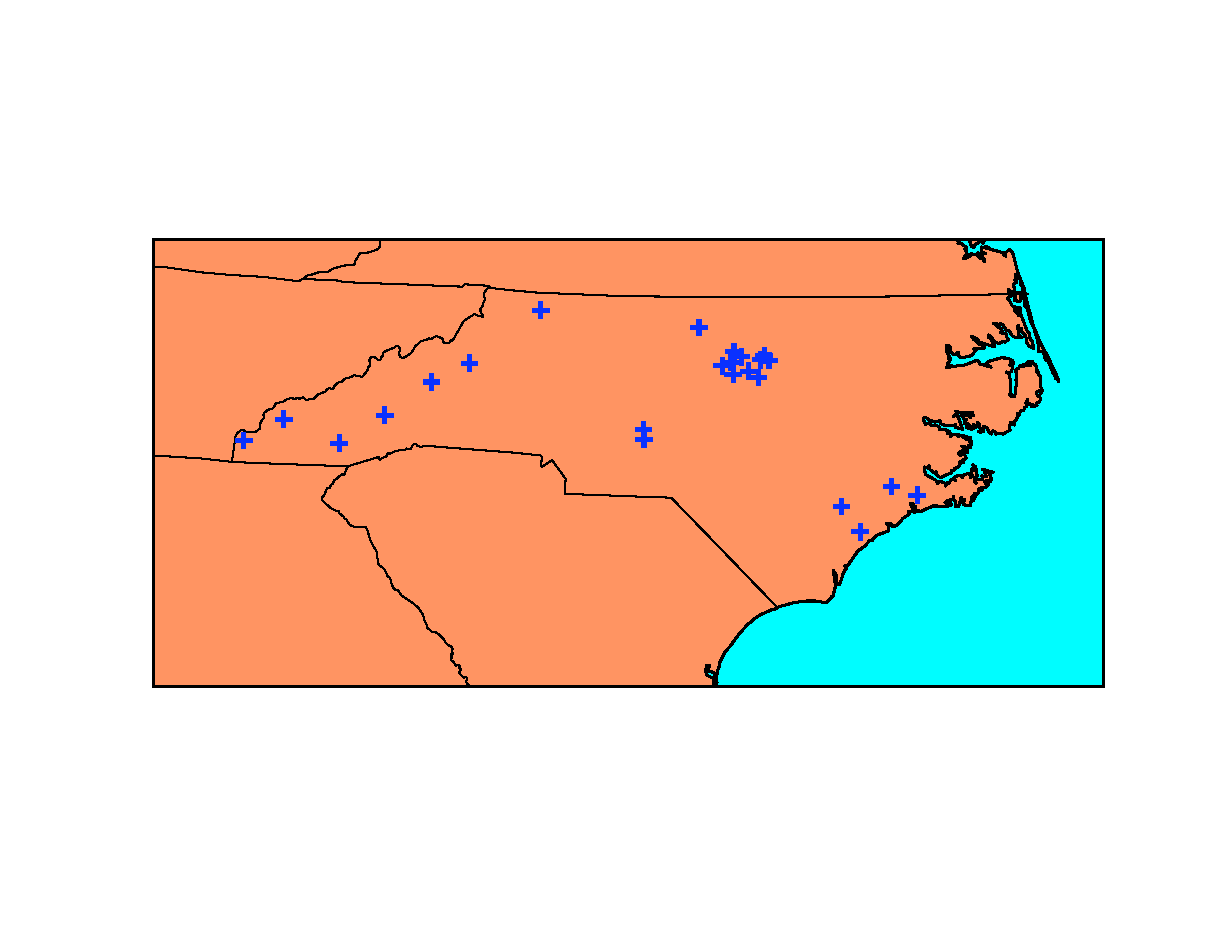
\includegraphics{lecture-03/mapfig.pdf}
\caption{Output of the mapex2.py module}
\end{figure}

\end{document}
